% UTF-8

% single-chapter commands
\documentclass[../main/thesis.tex]{subfiles}
\onlyinsubfile{\setcounter{chapter}{3}}  % single-chapter command
\begin{document}


\chapter{Algorithmen zur Generalisierung}

\section{Vorgehensweise}

...

% Erst über Generalisierung nachgedacht, da sie das schwierigerer Problem zu sein schien (in der Erwartung, die Identifikation ließe sich evtl. "nebenbei" lösen).
% Die Generalisierung ist auf den allerersten Blick ein einfaches geometrisches Problem, das keiner ausgefeilten Algorithmen a la 2.5 bedarf. Erst mal probiert, ob es sich so lösen lässt. Später festgestellt (-> Implementierung?), dass es in der Tat nicht so schrecklich schwierig war, jedoch die Entscheidung, was zusammengehört und was nicht, im Allgemeinen Fall schwieriger als erwartet war (ein Problem, das allerdings wohl auch für die Lösungen aus 2.5 bestanden hätte, womöglich gar in verstärktem Ausmaß).

% damals sehr früh (noch vor Anmeldung) den Algorithmus in groben Zügen aufgestellt und implementiert
% Vorgehen war im Prinzip, das Problem graphisch/geometrisch anzugehen und auf Papier zu lösen, dann in Code zu übertragen
% anschließend nur noch (sehr umfangreiche) Verbessserungen vorgenommen, insbesondere zur Flexibilisierung (individuellere Analyse, unterschiedliche Testdaten, Spezialfälle)
% zeitaufwändig: Alg. implementieren; insb.: Probleme im Workflow lösen (z. B. I/O), OOP, die Details des Alg. so hinbekommen, dass er halbwegs "rund" läuft, Probleme wie bei Kreuzungen
% habe versucht, ein wenig Test-Driven Development zu lernen, was mir schwer fiel, weil ich ständig die Struktur änderte
% erst versucht, rein geometrisch zu arbeiten, dann festgestellt (mit Jochen), dass bei Autobahnen etc Tags idR passen und die Sache erleichtern

% an dieser Stelle außerdem big picture: wie hängen die folgenden teile zusammen?
% -> lt. Themenblatt soll das Analyseergebnis auch separat von der Generalisierung zu verwenden sein!
% d.h. die Main-Klasse / Fassade sollte gar nicht hier beschrieben werden, das ist ein Implementierungsdetail (unter Kap. 5 zu beschrieben, wozu aber Kap. 5 wohl etwas umorganisiert werden müsste)
% anstatt des Analyser-Outputs ist tatsächlich bisher der CorrelationGraph das Analyseergebnis, jedoch noch unvollständig (man bräuchte noch eine Art Metrik, dass z. B. ab 80% parallelen Segmenten zwei Ways als parallel gelten; evtl. auch einen Append-Schritt, denn zur (verlangten) Identifikation paralleler Linienzüge müssten diese erst mal aus den Ways erzeugt werden, falls die Ways nicht ausreichen)

% im CLI sieht's im Moment in etwa so aus:
% 1. create OsmDataset (als InputDataset-Instanz, via ShapeReader)
% 2. Combiner.run
% 3. output
% also eigentlich nichts, was algorithmisch einer besonderen Beschreibung bedarf

% an dieser Stelle außerdem __Überleitung__: was kann man aus 2.5 für lehren/erkenntnisse ziehen? irgendwas anwendbares dabei? wenn ja, warum nicht?


\section{Beschreibung der Algorithmen}

Im Folgenden werden die gefundenen Algorithmen zunächst in allgemeinen Begriffen beschrieben, wobei der Fokus auf ihrem Zusammenwirken und ihren Abhängigkeiten voneinander liegt. Im Anschluss daran folgt ihre formale Beschreibung.

% erst Grundprinzip beschreiben, dann Edge Cases

\subsection{Grundprinzip}

Um das Zusammenfassen paralleler Linienzüge vorzubereiten, werden alle \term{nodes} des einen Linienzugs jeweils einem gegenüberliegenden \term{node} auf dem parallelen Linienzug zugeordnet.
Die Verbindung der Mittelpunkte zwischen den einander zugeordneten \term{nodes} ergibt direkt den zusammengefassten Linienzug (Abbildung~\ref{fig:general-approach}).

Dieses Vorgehen vermeidet, dass die in Abschnitt~\ref{osm-fragmentation} besprochene häufige ungleichmäßige Fragmentierung von \osm-Linienzügen in mehrere \term{ways} einen Einfluss auf den Generalisierungsvorgang hat.
Aufgrund der ungleichen Verteilung der \term{nodes} kommt es vor, dass ein \term{node} des einen Linienzugs mehreren \term{nodes} des anderen Linienzugs zugeordnet wird, was jedoch unproblematisch ist.

\begin{figure}[ht]
  \begin{minipage}[t]{.5\linewidth}
    \centering
    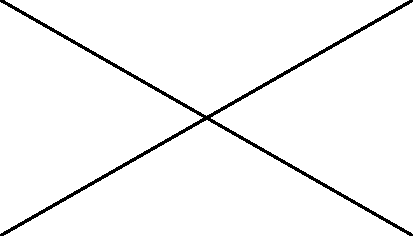
\includegraphics[width=\ScaleIfNeeded]{../image-missing}
    \caption{general-approach}\label{fig:general-approach}
  \end{minipage}%
  \begin{minipage}[t]{.5\linewidth}
    \centering
    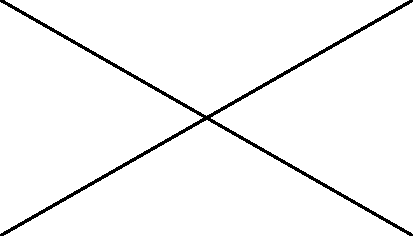
\includegraphics[width=\ScaleIfNeeded]{../image-missing}
    \caption{motorway-fragments}\label{fig:motorway-fragments}
  \end{minipage}
\end{figure}

Um zwei gegenüberliegende \term{nodes} einander zuordnen zu können, müssen zunächst die Linien, deren Teil sie sind, als zueinander parallel erkannt werden.
Auch hierbei ist die erwähnte ungleichmäßige Fragmentierung in bestimmten Fällen problematisch.
Beispielsweise müssten die einzelnen \term{ways} in Abbildung~\ref{fig:motorway-fragments}, aus denen die beiden dargestellten Parallelen bestehen, zunächst zu einem längeren Linienzug verknüpft werden, um einen Vergleich zu ermöglichen.
Dies entspräche dem in Abschnitt~\ref{os-mastermap} beschriebenen Ansatz von Thom, der damit zufriedenstellende Resultate erzielte, dabei jedoch die hohe Qualität seiner Ausgangsdaten betonte, welche bei wie für \osm{} von Freiwilligen erfassten Geodaten nicht vorausgesetzt werden kann.
% lässt sich diese aussage belegen?

Um diese Problematik zu umgehen, verwenden die in dieser Arbeit vorgestellten Algorithmen möglichst \emph{kurze} Liniensegmente anstelle möglichst \emph{langer} Linienzüge.
Die Verbindung zweier benachbarter \term{nodes} in einem \term{way} als kürzestmögliche lineare Einheit in den \osm-Ausgangsdaten (früher als \term{segment} bezeichnet) ist allerdings für einen Vergleich nicht viel besser geeignet als der vollständige \term{way} (Abbildung~\ref{fig:motorway-fragments}).
% warum nicht?
Daher werden die \term{segments} für die Analyse auf Parallelität zunächst solange immer weiter unterteilt, bis schließlich ein einfacher geometrischer Vergleich möglich ist.





% alte Einteilung:

\subsection{Identifikation parallel verlaufender Linien-Fragmente}

Ansatz: Dieser Algorithmus eignet sich insgesamt weniger gut zur Identifikation als zur Generalisierung. Die Identifikation erfolgt, indem festgestellt wird, ob eine Generalisierung notwendig ist oder nicht; falls sie notwendig ist, kann sie dann aber auch bereits recht billig durchgeführt werden. Andererseits ist fraglich, welchen "praxistauglichen" Einsatz eine reine Identifikation ohne anschließende Generalisierung hätte.

Konzept (abstrakt):

1. nur Segmente betrachten (gerade Linienabschnitte, definiert durch zwei Punkte)

2. alle nahe beieinander liegenden Segmente auf Parallelität untersuchen

Die Segmente sind jedoch unterschiedlich lang und liegen teilweise etwas „verstreut“ im Raum, was die Untersuchung erschwert.
Deshalb werden die Segmente zunächst fragmentiert, indem benachbarte Segmente „geschickt“ weiter in kürzere Segmente unterteilt werden, so dass parallele Segmente immer ähnlich lang sind und einander gegenüberstehen.

Im Detail:

1. geometrische Indizierung (R-Tree) der Eingabedaten, um Suche nach nahen LineParts zu ermöglichen [regionalise]

2. $\forall$ LineParts: AbstractLinePart.splitCloseParallels, um gut vergleichbare Stücke zu erhalten (reentrant/rekursiv, d. h. neu erzeugte Fragmente werden bis zu einer Mindestgröße immer weiter aufgeteilt) [split]

3. $\forall$ LineParts: $\forall$ nahe Parallelen (laut Index): [analyse]

3.1 Vorprüfung (boolean)

3.2 Hauptprüfung (double)

3.3 best matches (links/rechts getrennt) speichern (keine Nachprüfung => falls das best match nicht passt, wird es trotzdem genommen, sofern nicht schon die vorprüfung die sache abgebrochen hat)
% offen: "realParallels"-Konzept
% geprüft werden die Fragmente, gespeichert werden die Segmente

% graphisch erklären, was genau passiert


\subsection{Generalisierung durch Zusammenfassung}

Konzept (in den allgemeinsten Begriffen):

1. Endpunkte der parallelen Segmente einander zuordnen

2. Der gesamte Graph wird "durchgehangelt", indem von einer CorrelationEdge ausgehend immer entlang der Segmente das nächste CorrelationEdge gefunden wird; diese Edges werden dann durch neu erzeugte Mittelpunkte miteinander verbunden.



% (Der CorrelationGraph ist ein Graph, in dem CorrelationEdges einander gegenüberliegende Knoten von parallelen Segmenten verbinden.)

% new GeneralisedLines
% - beliebige CorrelationEdge auswählen und von ihr ausgehend den angrenzenden Segmenten erst in die eine, dann die andere Richtung folgen, bis das Folgen nicht mehr eindeutig möglich ist (z. B. wegen einer Abzweigung)
% - dabei Mittelpunkte der CorrelationEdges jeweils einer neuen GeneralisedSection hinzufügen
% - Segmente, die nicht zusammengefasst wurden (weil keine Parallelen existieren), werden in Sections umgewandelt und ebenfalls den GeneralisedLines hinzugefügt, um einen homogenen Ergebnisdatensatz zu erhalten

...


\subsection{Verknüpfung von Linienfragmenten zu einem einzigen kontinuierlichen Linienzug}

...


% single-chapter commands
%\onlyinsubfile{\listoffigures} \onlyinsubfile{\listoftables}
%\onlyinsubfile{% global bibliography settings

\nocite{*}  % include works in bibliography that aren't cited anywhere in the document (for debugging)

\setbibpreamble{Die Literaturangaben sind alphabetisch nach den Nachnamen der Autoren sortiert. Bei mehreren Autoren wird nach dem ersten Autor sortiert.\par\bigskip\bigskip}

\bibliography{../references-papers,../references-manual}
%\bibliography{../references-manual}
}
\end{document}
